\section{Validazione e Test}
Il sito � stato concepito per sfruttare appieno le potenzialit� dei browser moderni, al fine di offrire un'esperienza quanto pi� simile ad un'applicazione nativa. Ad esempio, in alcune sezione del sito sono state implementate finestre di dialogo e una navigazione "refreshless" (senza ricaricamenti delle pagine), non voltando le spalle alla retrocompatibilit�. Nello specifico, quindi, il sito � supportato dai seguenti browser\footnote{ Le ultime versioni si riferiscono a quelle presenti al momento della stesura della relazione (29/06/2018)}\footnote{ Testati su Windows 10 64 bit, Ubuntu 16.04 64 bit, Ubuntu 18.04 64 bit}: 
\begin{itemize}
	\item Google Chrome da versione 42 a versione 67 
	\item Internet Explorer da versione 8 inclusa
	\item Microsoft Edge da versione 13
	\item Mozilla Firefox da versione 10.0.1(ESR) a versione 60
	\item Opera
	\item Browser integrato Andorid da versione 4.0 del sistema operativo
	\item Safari mobile da versione 9.3.x del sistema operativo iOS
	
\end{itemize}
\begin{figure}[h]
	\footnotesize
	\centering
	\textbf{Versione mobile}\par\medskip
	\stackunder[5pt]{
\includegraphics[scale=0.25]{images/android_home1.jpg}}{Home} \qquad
	\hspace{1cm}%
	\stackunder[5pt]{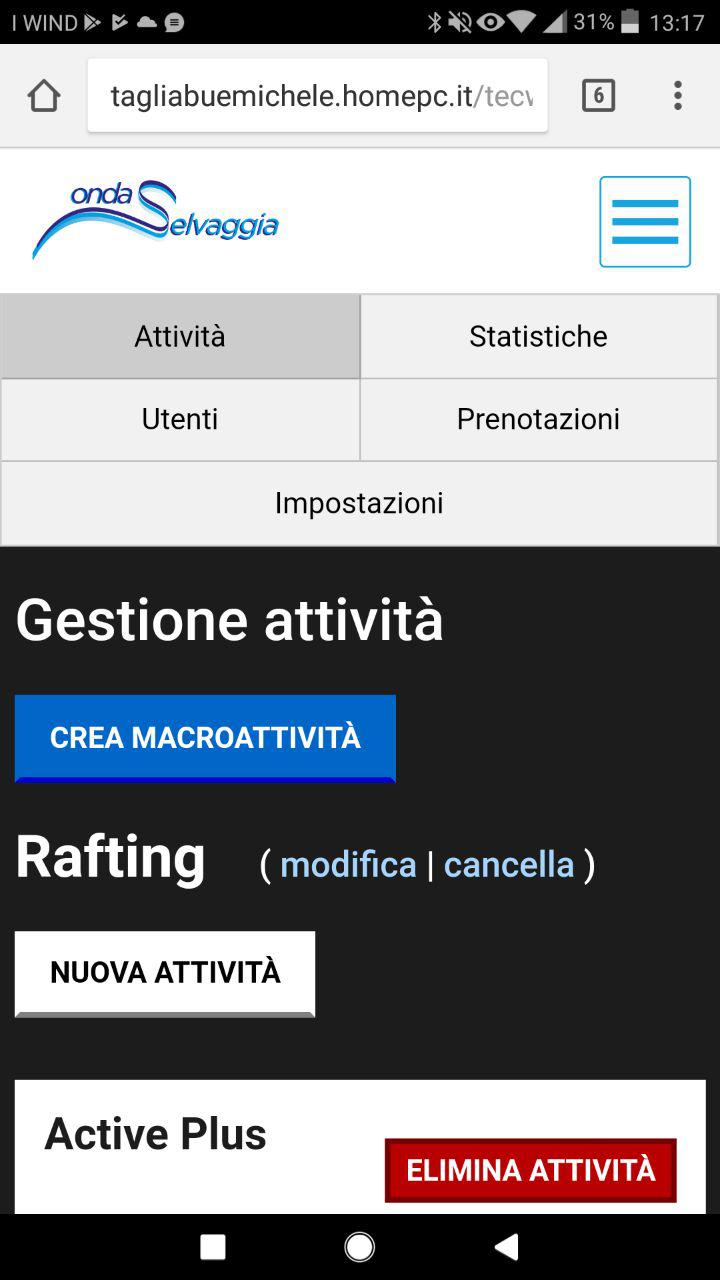
\includegraphics[scale=0.25]{images/android_admin.jpg}}{Pannello Admin} \\
\end{figure}
Non si riportano immagini dei vari test sui diversi browser desktop poich� non ci sono sostanziali differenze a livello grafico e di usabilit�.